\documentclass[12pt,a4paper]{article}
\usepackage[utf8]{inputenc}
\usepackage[english]{babel}
\usepackage[T1]{fontenc}
\usepackage{amsmath}
\usepackage{amsfonts}
\usepackage{amssymb}
\usepackage{graphicx}
\usepackage{siunitx}
\usepackage{float}
\usepackage[left=2cm,right=2cm,top=2cm,bottom=2cm]{geometry}
\author{Gerald}

\begin{document}
\sisetup{separate-uncertainty = true}
	\setlength{\parindent}{0pt} 
	\begin{center}
		{\LARGE Experiment protocol}\\
		\begin{large}
			for the solid state lab course\\[0.4cm]
			at RWTH Aachen\\
			II. Physikalisches Institut A\\[5.5cm]
			\Large\textbf{\textsl{Quantum Transport}}\\[5.5cm]
			\normalsize\textit{authored\\by}\\[0.4cm]
			\large{Moritz Berger (355244)\\Gerald Kolter (355005)}\\[2cm]
			\large \textbf{Summer term 2019}
		\end{large}
	\end{center}
	\newpage
	
	\tableofcontents
	\newpage

\section{Introduction}
At the interfaces between different materials the fermi levels align. Therefor the conduction and valence band bend. One can use this effect to create a two dimensional electron gas ("2DEG"). This is done by building a sample of thin layers of different materials. If done correctly, the conduction band bends underneath the Fermi level in one of the layer and is above it in every other layer. \\
With this structure one builds a hall probe, meaning a rectangular sample through which a current flows from side to side. The resistivity of the sample is measured parallel and perpendicular to this current. A variable magnetic field is applied perpendicular to the 2DEG. \\
At low temperatures the density of states in the 2DEG at zero magnetic field is a simple step function. With applying a magnetic field Landau levels are formed meaning the density of states becomes a function with single peaks, whose height, width and distance to each other depend on the magnetic field. As the Fermi energy stays the same, the density of states at the Fermi energy oscillates with the magnetic field. And as the resistivity depends mainly on the density of states at the Fermi energy the resistivity parallel to the magnetic field oscillates as well. These oscillations are called "Shubnikov-de Haas oscillations". \\
The resistivity perpendicular to the magnetic field depends linearly on the magnetic field and builds Hall plateaus.


\section{Goal of the Experiment}
The goal of the experiment is to determine different properties of the 2DEG: The charge carrier concentration $n_s$, the effective electron mass $m^*$, the quantum relaxation time $\tau _q$, the transport relaxation time $\tau _{tr}$ and the effective electrons' g-factor.


\section{Setup}
The 2DEG is build between a layer of GaAs and a layer of Al$_{x}$Ga$_{1-x}$As. For applying a magnetic field an electromagnet build from a superconductor is used. For the cooling a custom build cryostat is used. It consists out of an inner liquid helium (LHe) bath in which the sample is sunk. The LHe is sunk in an outer liquid nitrogen (LN) bath. Between these two an inner vacuum insulation and around the LN an outer vacuum insulation is formed for reducing heat conductance. \\
With this setup one can cool down the sample to \SI{4.2}{K}. To reach lower temperatures one pumps the gaseous helium out of the inner tube. With this one reaches the triple point of helium at around \SI{2.2}{K}.


\section{Measurement}
The magnetic field is sweeped from \SI{-5.4}{T} to \SI{5.4}{T}. Meanwhile the resistivity parallel and perpendicular to the current is measured. This is done at without pumping, meaning at about \SI{4.2}{K}, with a fractional pumping power, meaning at about \SI{3.5}{K}, and with maximal pumping power, meaning at about \SI{2.2}{K}.

\subsection{Data}

\begin{figure} [H]
\centering
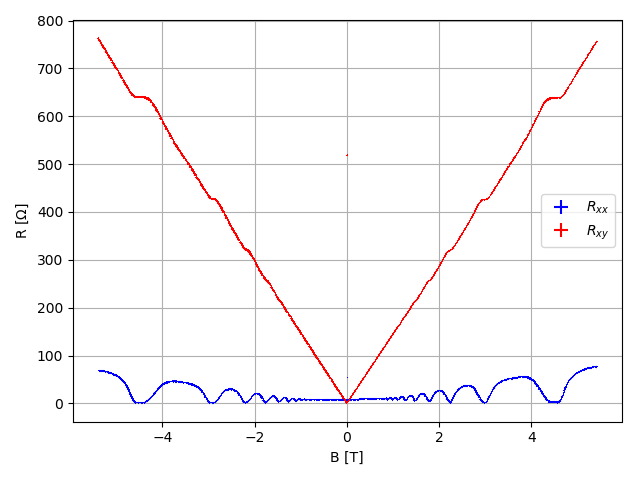
\includegraphics[scale=0.8]{Bilder/Elektron_g/4_2/Rohdaten.PNG}
\caption{Measured resistivities $R_{xx}$ and $R_{xy}$ in dependence of the magnetic field at \SI{4.2}{K}.}
\label{fig:raw_data}
\end{figure}

Fig. \ref{fig:raw_data} shows the measured raw data for the resistivities $R_{xx}$ and $R_{xy}$ in dependence of the magnetic field exemplary at \SI{4.2}{K}. The measurements at \SI{3.5}{K} and \SI{2.2}{K} yield similar results.



\section{Charge carrier concentration}
\subsection{Data analysis}
The charge carrier concentration can be extracted from the SdH-oscillations. It is given by
\begin{equation}
n_s = g_s g_v \dfrac{e}{h} \left(\dfrac{1}{B_{i+1}} - \dfrac{1}{B_{i}}\right)
\end{equation}
with $g_s = 2$ and $g_v = 1$ for our sample. The last part of this equation describes the distance between two oscillation minima. This is equivalent to one oscillation period when plotting the data against $1/B$,which van be seen in figure \ref{fig:n_inverseB}. In order to determine the period a FFT-analysis of the data is performed.\\
In a first step the data where $|B| < \SI{0.1}{T}$ is ignored to avoid large numbers in the $1/B$ plot and to achieve a cleaner Fourier-analysis. The data is then interpolated to achieve equivalent spacing in the $1/B$ plot. The FFT-analysis is performed separately for the positive and negative magnetic field for each measurement. One of the resulting frequency spectra can be seen in figure \ref{fig:n_FFT}. The spectrum shows a peak at about \SI{9}{T^{-1}}. In order to get a quantitative value the position of the maximum value of this peak is extracted. The error is determined by the resolution of the Fourier-spectrum by assuming an equal distribution across the peak position and its neighboring discrete points. For the shown spectra of the positive part of the \SI{4.2}{K} measurement this results in a frequency of
\begin{equation*}
f = \SI{8.95(12)}{T^{-1}}
\end{equation*}
From this $n_s$ can be calculated:
\begin{equation}
n_s = g_s g_v \dfrac{e}{h} \dfrac{1}{f} = \SI{5.40(7)E9}{cm^{-2}}
\end{equation}
The carrier concentration can also be extracted from the Hall measurement Rxy by
\begin{equation}
R_{xy} = - \dfrac{B}{n_s e}
\end{equation}
For this the slope of the $R_{xy}$ curve is extracted by a linear fit to the data between $\SI{0.1}{T}$ and $\SI{1}{T}$. This area is chosen to minimize the impact of the Hall-plateaus, which are smaller for small fields. For the positive part of the \SI{4.2}{K} measurement this is shown in figure \ref{fig:n_xy} and results in a slope of
\begin{equation}
a = \SI{144.31(13)}{\Omega/T}
\end{equation}
from which $n_s^{Hall}$ can be extracted:
\begin{equation}
n_s^{Hall} = \dfrac{1}{a e} = \SI{4.325(4)E12}{cm^{-2}}
\end{equation}
The error comes directly from the fit.
\begin{figure}
\centering
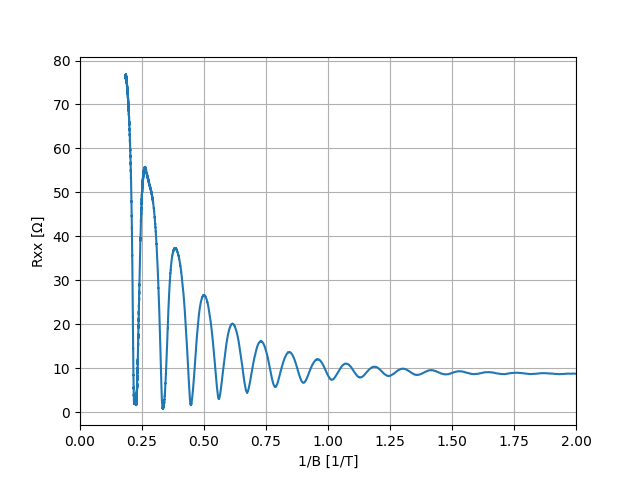
\includegraphics[scale=0.8]{Bilder/inverseB.png}
\caption{Rxx plotted against the inverse magnetic field to visualize the oscillations. Only the positive part is shown.}
\label{fig:n_inverseB}
\end{figure}

\begin{figure}
\centering
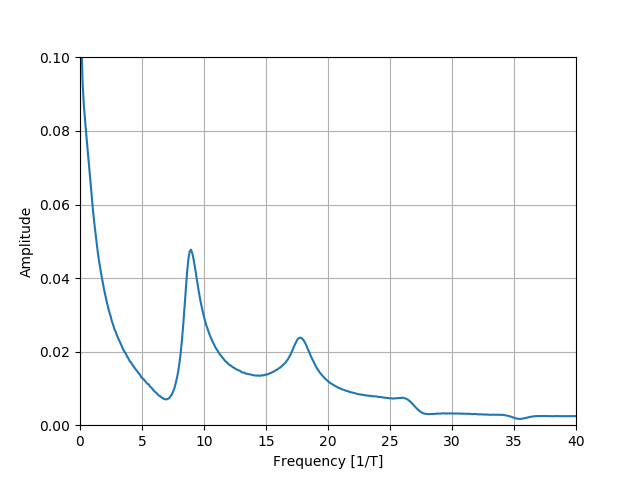
\includegraphics[scale=0.8]{Bilder/FFT4_2.png}
\caption{FFT-analysis of the part with positive magnetic field from the \SI{4.2}{K} measurement. The amplitude is normed to the highest peak. The SdH-socillation frequency shows in a peak at about \SI{9}{T^{-1}}.}
\label{fig:n_FFT}
\end{figure}

\begin{figure}
\centering
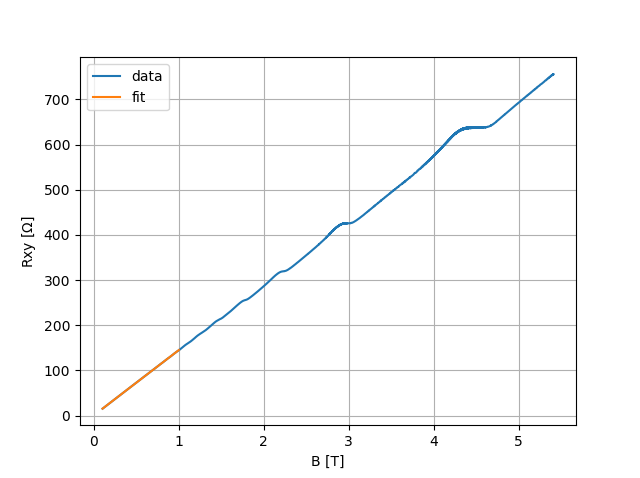
\includegraphics[scale=0.8]{Bilder/Rxy_fit.png}
\caption{linear fit to the $R_{xy}$ data in order to extract the slope.}
\label{fig:n_xy}
\end{figure}


\subsection{Results}

The results for the carrier concentration extracted from the SdH-oscillations for all three measurements are listed in table \ref{tab:n}. The weighted mean of these values results in a final value of
\begin{equation*}
n_s^{SdH} = \SI{5.35(7)e9}{cm^{-2}}
\end{equation*}
The concentrations extracted from the Hall measurements are listed in table \ref{tab:n_hall} with a weighted mean of
\begin{equation*}
n_s^{Hall} = \SI{4.36(7)e12}{cm^{-2}}
\end{equation*}

\begin{table} [H]
\centering
\begin{tabular}{|c|c|c|}
\hline 
measurement at & positive sign [\SI{e9}{cm^{-2}}] & negative sign [\SI{e9}{cm^{-2}}] \\ 
\hline 
$\SI{4.2 \pm 0.01}{K}$ & $5.40\pm 7$ & $5.38\pm 7$ \\ 
\hline 
$\SI{3.38 \pm 0.17}{K}$ & $5.38\pm 7$ & $5.29\pm 7$ \\ 
\hline 
$\SI{2.329 \pm 0.087}{K}$ & $5.23\pm 7$ & $5.43\pm 7$ \\ 
\hline 
\end{tabular} 
\caption{Measured values for the charge carrier concentration $n_s$ extracted from the oscillations}
\label{tab:n}
\end{table}

\begin{table} [H]
\centering
\begin{tabular}{|c|c|c|}
\hline 
measurement at & positive sign [\SI{e12}{cm^{-2}}] & negative sign [\SI{e12}{cm^{-2}}] \\ 
\hline 
$\SI{4.2 \pm 0.01}{K}$ & $4.325\pm 0.004$ & $4.240\pm 0.006$ \\ 
\hline 
$\SI{3.38 \pm 0.17}{K}$ & $4.392\pm 0.008$ & $4.346\pm 0.009$ \\ 
\hline 
$\SI{2.329 \pm 0.087}{K}$ & $4.436\pm 0.015$ & $4.424\pm 0.015$ \\ 
\hline 
\end{tabular} 
\caption{Measured values for the charge carrier concentration from the Hall measurement.}
\label{tab:n_hall}
\end{table}

\section{Effective electron mass}
\subsection{Data analysis and Results}
The effective mass can be extracted with the help of the following formula:
\begin{equation}
\dfrac{\Delta R_{xx}^{\pm}(B,T_1)}{\Delta R_{xx}^{\pm}(B,T_2)} = \dfrac{T_1 sinh(X(T_2))}{T_2 sinh(X(T_1))}
\label{eq:mass}
\end{equation}
where
\begin{equation}
X = \dfrac{2 \pi^2 k_b T}{\hbar \omega_c} = \dfrac{2 \pi^2 k_b T m^*}{\hbar e B} 
\end{equation}
$\Delta R_{xx}^{\pm}(B,T)$ denotes the difference of the envelope of the oscillations, which needs to be extracted from the measured data. This is done by determining the position of the first 15 maxima and minima of the oscillation and then fitting an exponential fit against them as seen in figure \ref{fig:m_fit}. Then the two fits are subtracted from each other in order to determine $\Delta R_{xx}^{\pm}(B,T)$. This is then done for a measurement with different temperature. We only analyze the positive part of the \SI{4.2}{K} and  \SI{2.2}{K} measurements, because the temperature gradient of the \SI{3.6}{K} measurement leads to a wrong result. The values of the exponential fits can be found in table \ref{tab:exp}. With these results the left part of equation \ref{eq:mass} can be plotted as seen in figure \ref{fig:m}. This is only done for $T_1 = \SI{4.2}{K}$ and $T_2 = \SI{2.2}{K}$.\\
In order to determine the effective mass a function similar to the right part of equation \ref{eq:mass} with $m^*$ as a parameter is fitted against the plot and optimized with the help of the least squares method. The error of $m^*$ is calculated by changing all parameters (including the temperatures) by their errors and calculating a new best value of $m^*$. The maximum difference between the new value and the original one denotes the error. The final result is 
\begin{equation*}
m^* = \SI{0.059 \pm 0.006}{m_e}
\end{equation*}

\begin{table}
\centering
\begin{tabular}{|c|c|c|c|}
\hline 
measurement at & parameter & $ R_{xx}^{+}(B,T)$ & $ R_{xx}^{-}(B,T)$ \\ 
\hline 
$\SI{4.2 \pm 0.01}{K}$ & $A_0$ & $129.96\pm 5.67$ & $-15.84\pm 1.83$ \\ 
\hline
$\SI{4.2 \pm 0.01}{K}$ & $b$ & $3.98\pm 0.07$ & $2.04\pm 0.20$ \\ 
\hline
\hline 
$\SI{3.38 \pm 0.17}{K}$ & $A_0$ & $135.64\pm 12.21$ & $-12.07\pm 1.12$ \\ 
\hline 
$\SI{3.38 \pm 0.17}{K}$ & $b$ & $3.66\pm 0.09$ & $1.12\pm 0.12$ \\ 
\hline 
\hline 
$\SI{2.329 \pm 0.087}{K}$ & $A_0$ & $128.05\pm 8.43$ & $-9.92\pm 0.73$ \\ 
\hline 
$\SI{2.329 \pm 0.087}{K}$ & $b$ & $3.02\pm 0.09$ & $0.51\pm 0.08$ \\ 
\hline 
\end{tabular} 
\caption{parameter describing the envelope of the form $y = A_0 e^{-b/B}$}
\label{tab:exp}
\end{table}

\begin{figure}
\centering
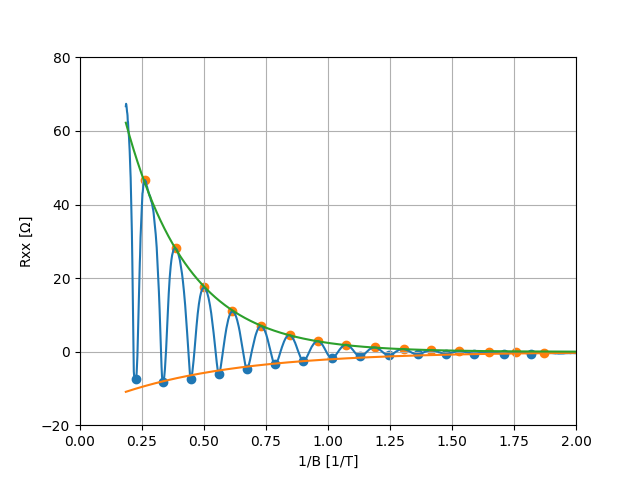
\includegraphics[scale=0.8]{Bilder/peaks.png}
\caption{Extracted maxima and minima and the exponential fit.}
\label{fig:m_fit}
\end{figure}

\begin{figure}
\centering
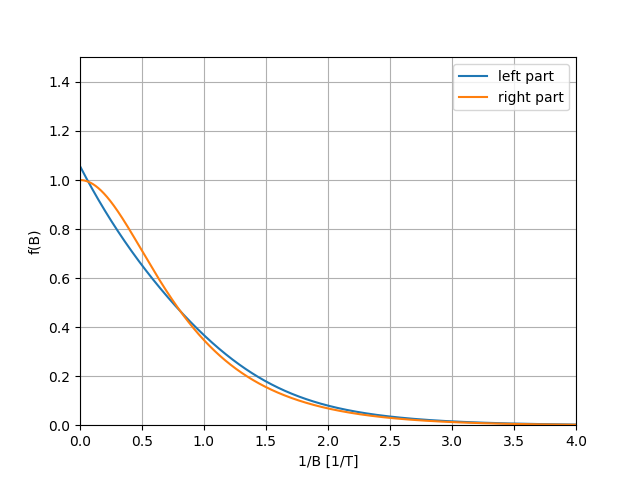
\includegraphics[scale=0.8]{Bilder/m.png}
\caption{left and right part of equation \ref{eq:mass} plotted with an optimized mass-parameter.}
\label{fig:m}
\end{figure}



\section{relaxation time}
\subsection{Data analysis}
By having calculated a value for the effective mass the quantum relaxation time can be extracted over the following equation
\begin{equation}
ln(\Delta R_{xx}^{\pm}(B,T)) \thicksim -\dfrac{\pi m^*}{e \tau_q} \dfrac{1}{B}
\end{equation} 
By plotting $ln(\Delta R_{xx}^{\pm}(B,T))$ over $1/B$ one can extract the slope, which determines $\tau_q$. The plot is shown in figure \ref{fig:tau}. The result is not completely linear and instead split into 2 linear regimes with a different slope. Because SdH-oscillations are only appear for large magnetic field (equating to small values in the plot) it is assumed that the linear regime ranging from 0 to about 1 is the correct one. A linear fit is fitted against this regime to extract its slope, which is also shown in figure \ref{fig:tau}. $\tau_q$ is then calculated from the extracted slope. The error is calculated by error propagation from the errors of the slope and the effective mass. This is done for each measurement.\\
\\
The transport relaxation time can be calculated with the help of the charge carrier concentration and the classical Hall effect:
\begin{equation}
R_{xx} = \dfrac{l}{w} \dfrac{m^*}{e^2 n_s \tau_{tr}}
\end{equation}
with the width $w \approx \SI{200}{\mu m}$ and length $l \approx \SI{500}{\mu m}$.
$R_{xx}$ is extracted by determining the value for $B = \SI{0}{T}$ from the data. This is done by averaging the data points between $|B|<0.5$. The error of $R_{xx}$ is derived from the standard derivation of the data points. From this $\tau_{tr}$ can be directly calculated using $n_s^{Hall}$ from the previous analysis.


\begin{figure}
\centering
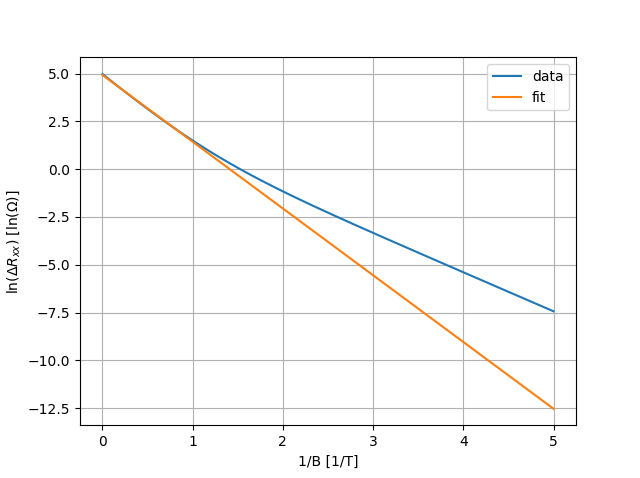
\includegraphics[scale=0.8]{Bilder/tau.png}
\caption{}
\label{fig:tau}
\end{figure}

\subsection{Results}

The extracted quantum relaxation times are listed in table \ref{tab:tau_q}. The weighted mean leads to a final result of
\begin{equation*}
\tau_q = \SI{0.36(5)}{ps}
\end{equation*}
The results for the transport relaxation time are listed in table \ref{tab:tau_tr}. The weighted mean leads to
\begin{equation*}
\tau_{tr} = \SI{2.48(17)}{ps}
\end{equation*}
As expected $\tau_{tr}$ is larger than $\tau_{q}$.

\begin{table}
\centering
\begin{tabular}{|c|c|c|}
\hline 
measurement at & a & $\tau_q$ [ps]\\ 
\hline 
$\SI{4.2 \pm 0.01}{K}$ & $-3.493 \pm 0.003$ & $0.30\pm 0.03$ \\ 
\hline
$\SI{3.38 \pm 0.17}{K}$ & $-3.020 \pm 0.005$ & $0.35\pm 0.04$ \\ 
\hline
$\SI{2.329 \pm 0.087}{K}$ & $-2.455 \pm 0.004$ & $0.43\pm 0.04$ \\ 
\hline
\end{tabular} 
\caption{Results for the extracted slope and the quantum relaxation time for different temperatures.}
\label{tab:tau_q}
\end{table}

\begin{table}
\centering
\begin{tabular}{|c|c|c|}
\hline 
measurement at & $R_{xx}[\Omega]$ & $\tau_tr$ [ps]\\ 
\hline 
$\SI{4.2 \pm 0.01}{K}$ & $7.98 \pm 0.25$ & $2.40\pm 0.25$ \\ 
\hline
$\SI{3.38 \pm 0.17}{K}$ & $7.64 \pm 0.20$ & $2.51\pm 0.27$ \\ 
\hline
$\SI{2.329 \pm 0.087}{K}$ & $7.27 \pm 0.74$ & $2.63\pm 0.38$ \\ 
\hline
\end{tabular} 
\caption{Results for the transport relaxation time at different temperatures.}
\label{tab:tau_tr}
\end{table}


\section{Electrons effective g-factor}
\subsection{Data analysis}
The resistivity of the minima of the Shubnikov-de Haas oscillation follows an Arrhenius law:
\begin{equation*}
\sigma _{xx} = \sigma _0 \cdot e^{- \frac{\Delta _{xx}}{2 k_B T}} \qquad \Leftrightarrow \qquad R _{xx} = R _0 \cdot e^{\frac{\Delta _{xx}}{2 k_B T}}
\end{equation*}
One can reformulate that to:
\begin{equation*}
\ln (R _{xx}) = \dfrac{\Delta _{xx}}{2 k_B T} + \ln (R _{0})
\end{equation*}
If the filling factor of the Hall probe is odd, the activation energy $\frac{\Delta _{xx}}{2}$ equals the Zeeman energy $g^* \mu _B B$ and so one gets:
\begin{equation*}
\ln (R _{xx}) = g^* \cdot \dfrac{\mu _B B}{k_B T} + \ln (R _{0})
\end{equation*}
Obviously one can determine the electrons effective g-factor as slope if one plots $\ln (R _{xx})$ on the y-axis and $\frac{\mu _B B}{k_B T}$ on the x-axis. \\
To extract the minima one determines the minima with a peak determination algorithm. With this one determines the B-field and the resistivity of the minimum as mean value of all datapoints which differ less than \SI{15}{\Omega} from the peak. The error is determined as the standard deviation of these datapoints. \\
This analysis is done with each measurement once with the part with positive magnetic field and once with the part with negative magnetic field.


\subsection{Results}

\begin{figure} [H]
\centering
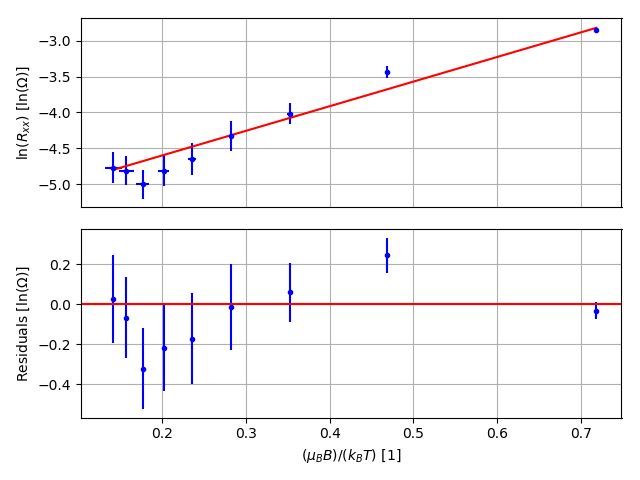
\includegraphics[scale=0.8]{Bilder/Elektron_g/4_2/lin_fit_Arrhenius_law_1.PNG}
\caption{Linear fit of the data to the Arrhenius law exemplary for the measurement at \SI{4.2}{K} and the part with positive sign.}
\label{fig:g-factor_lin_fit}
\end{figure}

Fig. \ref{fig:g-factor_lin_fit} shows exemplary the linear fit of the data to the Arrhenius law for the part with positive magnetic field of the measurement at \SI{4.2}{K}.

\begin{table} [H]
\centering
\begin{tabular}{|c|c|c|}
\hline 
 & positive sign & negative sign \\ 
\hline 
measurement at \SI{4.2}{K} & 3.44 $\pm$ 0.23 & 5.14 $\pm$ 0.37 \\ 
\hline 
measurement at \SI{3.5}{K} & 3.83 $\pm$ 0.28 & 4.91 $\pm$ 0.17 \\ 
\hline 
\end{tabular} 
\caption{Measured values for the effective electrons g-factor.}
\label{tab:electron_g_factor}
\end{table}

Tab. \ref{tab:electron_g_factor} lists all determined values for the effective electrons g-factor. As one averages these one gets as result:
\begin{equation*}
g^* = 5555 \pm 5555
\end{equation*}



\section{Conclusion}












\end{document}